\documentclass[a4paper,11pt,exos]{nsi} % COMPILE WITH DRAFT
\usepackage{pifont}
\usepackage{fontawesome5}

\begin{document}
\classe{\premiere spé}
\titre{Corrigé des exercices du cours}
\maketitle

\begin {exercice}
\begin{enumerate}
	\item Vérifier que $31$ est une solution de $10x-11 = 8x +51$.
	\item Vérifier que $7$ est une solution de $\dfrac{3}{4}x+\dfrac{2}{5}=\dfrac{3}{2}x-\dfrac{97}{20}$.
	\item Vérifier que $\sqrt{2}$ est une solution de $\sqrt{2}x-\sqrt{6}=-\sqrt{3}x+2$.	
\end{enumerate}
\end {exercice}

\begin{enumerate}
    \item \begin{multicols}{2}
    D'une part :
    \begin{tabbing}
        $10\times 31-11$\=$=310-11$\\
        \>$=299$
    \end{tabbing}
    D'autre part :
    \begin{tabbing}
        $8\times 31+51$\=$=248+51$\\
        \>  $=299$
    \end{tabbing}
    \end{multicols}
    Donc 31 est bien solution de l'équation $10x-11 = 8x +51$.
    
    \item \begin{multicols}{2}
        D'une part :
        \begin{tabbing}
            $\dfrac{3}{4}\times 7+\dfrac{2}{5}$\=$=\dfrac{21}{4}+\dfrac{2}{5}$\\[.5em]
            \>$=\dfrac{21\times 5}{4\times 5}+\dfrac{2\times 4}{5\times 4}$\\[.5em]
            \>$=\dfrac{105}{20}+\dfrac{8}{20}$\\[.5em]
            \>$=\dfrac{113}{20}$
        \end{tabbing}
        D'autre part :
        \begin{tabbing}
            $\dfrac{3}{2}\times 7-\dfrac{97}{20}$\=$=\dfrac{21}{2}-\dfrac{97}{20}$\\[.5em]
            \>  $=\dfrac{21\times 10}{2\times 10}-\dfrac{97}{20}$\\[.5em]
            \>  $=\dfrac{210}{20}-\dfrac{97}{20}$\\[.5em]
            \>  $=\dfrac{113}{20}$
        \end{tabbing}
        \end{multicols}
        Donc 7 est bien solution de l'équation $\dfrac{3}{4}x+\dfrac{2}{5}=\dfrac{3}{2}x-\dfrac{97}{20}$.

        \item \begin{multicols}{2}
            D'une part :
            \begin{tabbing}
                $\sqrt{2}\times \sqrt{2}-\sqrt{6}$\=$=\left(\sqrt{2}\right)^2-\sqrt{6}$\\[.5em]
                \>  $=2-\sqrt{6}$
            \end{tabbing}
            D'autre part :
            \begin{tabbing}
                $-\sqrt{3}\times \sqrt{2}+2$\=$=-\sqrt{2\times 3}+2$\\
                \>  $=2-\sqrt{6}$
            \end{tabbing}
            \end{multicols}
            Donc $\sqrt{2}$ est bien solution de l'équation $\sqrt{2}x-\sqrt{6}=-\sqrt{3}x+2$.
\end{enumerate}


\begin {exercice}
Résoudre les équations suivantes :
\begin{multicols}{2}
	\begin{enumerate}
		\item 	$34x-5=23x+50$
		\item 	$3x+1 = 3x -7$
		\item 	$2,4x-3=-5,7x+8$
		\item	$\displaystyle\frac{3}{4}x+1=\frac{7}{10}x-\frac{2}{7}$
		%\item	$\displaystyle\frac{1}{2}x+\dfrac{1}{3}=\frac{1}{4}x+\frac{1}{5}$
		\item 	$\sqrt{2}x-2=\pi x +\sqrt{5}$
		\item	$2x-3(4x-5)=17$
	\end{enumerate}
\end{multicols}
\end {exercice}

\begin{enumerate}
    \item \begin{tabbing}
        $34x-5=23x+50 \quad$  \=  $\iff \quad 34x-5\textcolor{UGLiOrange}{-23x}\textcolor{UGLiBlue}{+5}=23x+50\textcolor{UGLiOrange}{-23x}\textcolor{UGLiBlue}{+5}$\\
        \>  $\iff \quad 11x=55$\\
        \>  $\iff \quad \dfrac{11x}{\textcolor{UGLiOrange}{11}}=\dfrac{55}{\textcolor{UGLiOrange}{11}}$\\
        \>  $\iff \quad x=5$
    \end{tabbing}
    $\mathcal{S}_1=\left\{5\right\}$

    \item \begin{tabbing}
        $3x+1 = 3x -7 \quad$ \= $\iff \quad 3x+1 \textcolor{UGLiOrange}{-3x}= 3x -7 \textcolor{UGLiOrange}{-3x}$\\
        \>  $\iff \quad 1=-7$\\
        \>  $\phantom{\iff} \quad$ Cette égalité est toujours fausse.
    \end{tabbing}
    $\mathcal{S}_2=\varnothing \qquad$ Cette équation n'a pas de solution.

    \item \begin{tabbing}
        $2,4x-3=-5,7x+8 \quad$  \=  $\iff\quad 2,4x-3\textcolor{UGLiOrange}{+5,7x}\textcolor{UGLiBlue}{+3}=-5,7x+8\textcolor{UGLiOrange}{+5,7x}\textcolor{UGLiBlue}{+3}$\\
        \>  $\iff\quad 8,1x=11$\\
        \>  $\iff\quad  \dfrac{8,1x}{\textcolor{UGLiOrange}{8,1}}=\dfrac{11}{\textcolor{UGLiOrange}{8,1}}$\\
        \>  $\iff\quad x=\dfrac{110}{81}$
    \end{tabbing}
    $\mathcal{S}_3=\left\{\dfrac{110}{81}\right\}$

    \item \begin{tabbing}
        $\displaystyle\frac{3}{4}x+1=\frac{7}{10}x-\frac{2}{7}\quad$ \= 
        $\iff\quad \displaystyle\frac{3}{4}x+1 \textcolor{UGLiOrange}{-\dfrac{7}{10}x}\textcolor{UGLiBlue}{-1}=\frac{7}{10}x-\frac{2}{7}\textcolor{UGLiOrange}{-\dfrac{7}{10}x}\textcolor{UGLiBlue}{-1}$\\[.5em]
        \>  $\iff\quad \dfrac{3\textcolor{UGLiPurple}{\times 5}}{4\textcolor{UGLiPurple}{\times 5}}x-\dfrac{7\textcolor{UGLiPurple}{\times 2}}{10\textcolor{UGLiPurple}{\times 2}}x=-\dfrac{2}{7}-1$\\[.5em]
        \>  $\iff\quad \dfrac{15}{20}x-\dfrac{14}{20}x=-\dfrac{2}{7}-\dfrac{7}{7}$\\[.5em]
        \>  $\iff\quad \dfrac{1}{20}x=-\dfrac{9}{7}$\\[.5em]
        \>  $\iff\quad \dfrac{\textcolor{UGLiOrange}{20}}{20}x=-\dfrac{9\textcolor{UGLiOrange}{\times20}}{7}$\\[.5em]
        \>  $\iff\quad x=-\dfrac{180}{7}$
    \end{tabbing}
    $\mathcal{S}_4=\left\{-\dfrac{180}{7}\right\}$

    \item \begin{tabbing}
        $\sqrt{2}x-2=\pi x +\sqrt{5} \quad$ \=  $\iff\quad \sqrt{2}x -2 \textcolor{UGLiOrange}{-\pi x} \textcolor{UGLiBlue}{+2}=\pi x +\sqrt{5}\textcolor{UGLiOrange}{-\pi x}\textcolor{UGLiBlue}{+2}$\\[.5em]
        \>  $\iff\quad \sqrt{2}x-\pi x= \sqrt{5}+2$\\[.5em]
        \>  $\iff\quad \left(\sqrt{2}-\pi\right)x=2+\sqrt{5}$\\[.5em]
        \>  $\iff\quad \dfrac{\left(\sqrt{2}-\pi\right)x}{\textcolor{UGLiOrange}{\sqrt{2}-\pi}}=\dfrac{2+\sqrt{5}}{\textcolor{UGLiOrange}{\sqrt{2}-\pi}}$\\[.5em]
        \>  $\iff\quad x=\dfrac{2+\sqrt{5}}{\sqrt{2}-\pi}$
    \end{tabbing}
    $\mathcal{S}_5=\left\{\dfrac{2+\sqrt{5}}{\sqrt{2}-\pi}\right\}$

    \item \begin{tabbing}
        $2x-3(4x-5)=17 \quad$   \= $\iff\quad 2x-3\times 4x-3\times (-5)=17$\\
        \>  $\iff\quad 2x-12x+15=17$\\
        \>  $\iff\quad -10x+15\textcolor{UGLiOrange}{-15}=17\textcolor{UGLiOrange}{-15}$\\
        \>  $\iff\quad -10x=2$\\
        \>  $\iff\quad \dfrac{-10x}{\textcolor{UGLiOrange}{-10}}=\dfrac{2}{\textcolor{UGLiOrange}{-10}}$\\[.5em]
        \>  $\iff\quad x=-0,2$
    \end{tabbing}
    $\mathcal{S}_6=\left\{-0,2\right\}$
\end{enumerate}

\begin{exercice}[]
	Résoudre les équations suivantes :
	\begin{multicols}{2}
		\begin{enumerate}
			\item 	$(3x-5)(4x+8)=0$
			\item 	$x^2+3x-5=x^2-7x-4$
			\item	$(x-5)^2=(x+4)^2$
			\item	$(2x-1)(3x+2)+(2x-1)(7-x)=0$
			\item	$(4x-1)(x-7)-(x-7)^2=0$\\
				
		\end{enumerate}
	\end{multicols}
\end{exercice}

\begin{enumerate}
    \item \begin{tabbing}
        $(3x-5)(4x+8)=0 \quad$ \= $\iff \quad 3x-5=0\quad$ \= ou $\quad 4x+8=0$\\
        \>  $\iff \quad 3x=5$   \> ou $\quad 4x=-8$\\
        \>  $\iff \quad \dfrac{3x}{3}=\dfrac{5}{3}$ \> ou $\quad \dfrac{4x}{4}=-\dfrac{8}{4}$\\%[.5em]
        \>  $\iff \quad x=\dfrac{5}{3}$ \> ou $\quad x=-2$ 
    \end{tabbing}
    $\mathcal{S}_1=\left\{-2\ ;\dfrac{5}{3}\right\}$

    \item \begin{tabbing}
        $x^2+3x-5=x^2-7x-4\quad$    \= $\iff \quad x^2+3x-5 \textcolor{UGLiOrange}{-x^2}=x^2-7x-4 \textcolor{UGLiOrange}{-x^2}$\\
        \>  $\iff\quad 3x-5=-7x-4\qquad$\\
        \>  $\phantom{\iff}\quad$ \textit{On obtient une équation du premier degré.}\\
        \>  $\iff\quad 3x+7x=-4+5$\\
        \>  $\iff\quad 10x=1$\\
        \>  $\iff\quad \dfrac{10x}{10}=\dfrac{1}{10}$\\
        \>  $\iff\quad x=0,1$
    \end{tabbing}
    $\mathcal{S}_2=\left\{0,1\right\}$

    \item \textbf{Méthode 1 : En développant}
    \begin{tabbing}
        $(x-5)^2=(x+4)^2\quad$  \=  $\iff\quad x^2-2\times x\times 5+5^2=x^2+2\times x\times 4+4^2$\\
        \>  $\phantom{\iff}\quad$ \textit{On développe les identités remarquables.}\\
        \>  $\iff\quad x^2-10x+25\textcolor{UGLiOrange}{-x^2}=x^2+8x+16\textcolor{UGLiOrange}{-x^2}$\\
        \>  $\iff\quad -10x+25=8x+16$\\
        \>  $\iff\quad -10x-8x=16-25$\\
        \>  $\iff\quad -18x=-9$\\
        \>  $\iff\quad \dfrac{-18x}{-18}=\dfrac{-9}{-18}$\\
        \>  $\iff\quad  x=\dfrac{1}{2}$
    \end{tabbing}
    $\mathcal{S}_3=\left\{\dfrac{1}{2}\right\}$\\
\newpage
    \textbf{Méthode 2 : En factorisant}
    \begin{tabbing}
        $(x-5)^2=(x+4)^2\quad$  \=  $\iff\quad (x-5)^2-(x+4)^2=0$\\
        \>  $\phantom{\iff}\quad$ \textit{On reconnait une identité remarquable de la forme $a^2-b^2$.}\\
        \>  $\iff\quad \left((x-5)+(x+4)\right)\left((x-5)-(x+4)\right)=0$\\
        \>  $\phantom{\iff}\quad$ \textit{On factorise en $(a+b)(a-b)$.}\\
        \>  $\iff\quad (x-5+x+4)(x-5-x-4)=0$\\
        \>  $\iff\quad (2x-1)\times(-9)=0$\\
        \>  $\iff\quad \dfrac{(2x-1)\times(-9)}{-9}=\dfrac{0}{-9}$\\
        \>  $\iff\quad 2x-1=0$\\
        \>  $\iff\quad 2x=1$\\
        \>  $\iff\quad \dfrac{2x}{2}=\dfrac{1}{2}$\\
        \>  $\iff\quad  x=\dfrac{1}{2}$
    \end{tabbing}
    $\mathcal{S}_3=\left\{\dfrac{1}{2}\right\}$

    \item \begin{tabbing}
        $(2x-1)(3x+2)+(2x-1)(7-x)=0 \quad$ \= $\iff\quad (2x-1)\left[(3x+2)+(7-x)\right]=0$\\
        \>  $\iff\quad (2x-1)\left[3x+2+7-x\right]=0$\\
        \>  $\iff\quad (2x-1)(2x+9)=0$\\
        \>  $\iff\quad 2x-1=0\quad$ \= ou $\quad 2x+9=0$\\
        \>  $\iff\quad 2x=1$    \> ou $\quad 2x=-9$\\
        \>  $\iff\quad x=\dfrac{1}{2}$  \> ou $\quad x=-\dfrac{9}{2}$
    \end{tabbing}
    $\mathcal{S}_4=\left\{-\dfrac{9}{2}\ ; \dfrac{1}{2}\right\}$

    \item \begin{tabbing}
        $(4x-1)(x-7)-(x-7)^2=0 \quad$   \= $\iff\quad (4x-1)(x-7)-(x-7)(x-7)=0$\\
        \>  $\iff\quad (x-7)\left[(4x-1)-(x-7)\right]=0$\\
        \>  $\iff\quad (x-7)\left[4x-1-x+7\right]=0$\\
        \>  $\iff\quad (x-7)(3x+6)=0$\\
        \>  $\iff\quad x-7=0\quad$    \= ou $\quad 3x+6=0$\\
        \>  $\iff\quad x=7$  \> ou $\quad 3x=-6$\\
        \>  $\iff\quad x=7$ \> ou $\quad x=-2$
    \end{tabbing}
    $\mathcal{S}_5=\left\{-2\ ; 7\right\} $
\end{enumerate}

\begin {exercice}
Résoudre les inéquations suivantes et faire un schéma de l'ensemble des solutions.
\begin{multicols}{2}
	\begin{enumerate}
		\item 	$2x-5<7x-35$
		\item 	$3x+1 > -8x -7$
		\item 	$-1,2x-8,1>3,2x+5,7$
		\item 	$1,4x-3\geqslant-5,7x-18$
		\item	$\displaystyle\frac{2}{5}x+1\leqslant\frac{7}{10}x+\frac{2}{3}$
		\item	$\displaystyle\frac{3}{2}x+\dfrac{2}{3}>-\frac{1}{4}x+\frac{1}{5}$
	\end{enumerate}
\end{multicols}
\end {exercice}

\begin {exercice}
Donner le tableau de signes des expressions suivantes :
\begin{multicols}{2}
	\begin{enumerate}
		\item 	$3x+2$
		\item 	$-4x-9$
		\item 	$\dfrac{3}{5}x-\dfrac{2}{7}$
		\item 	$\sqrt{3}x-3$
		\item 	$(2x-1)(-3x+2)$
		\item	$\dfrac{5x-2}{-7x-8}$
	\end{enumerate}
\end{multicols}\ \\[-2em]
%Pour les deux dernières on étudiera le signe de chaque expression du premier degré puis on utilisera la règle des signes.
\end {exercice}

\begin{enumerate}
    \item \begin{multicols}{2}
        Calcul de la racine :
    \begin{tabbing}
        $3x+2=0\quad$   \=  $\iff\quad 3x=-2$\\
        \>  $\iff \quad x=-\dfrac{2}{3}$
    \end{tabbing}
    %\begin{center}
        \begin{tikzpicture}
            \tkzTabInit[color,lgt=4,espcl=1.5]
            {$x$ /1 ,signe de $3x+2$ /1}
            {$-\infty$, $-\dfrac{2}{3}$, $+\infty$ }
            \tkzTabLine{, - ,z,+,}
        \end{tikzpicture}
    %\end{center}
    \end{multicols}
    
    \item \begin{multicols}{2}
        Calcul de la racine :
        \begin{tabbing}
            $-4x-9=0\quad$  \=  $\iff\quad -4x=9$\\
            \>  $\iff\quad x=-\dfrac{9}{4}$
        \end{tabbing}       
        \begin{tikzpicture}
            \tkzTabInit[color,lgt=4,espcl=1.5]
            {$x$ /1 ,signe de $-4x-9$ /1}
            {$-\infty$, $\dfrac{9}{4}$, $+\infty$ }
            \tkzTabLine{, + ,z,-,}
        \end{tikzpicture} 
    \end{multicols}

    \item Calcul de la racine :
    \begin{multicols}{2}
        \begin{tabbing}
            $\dfrac{3}{5}x-\dfrac{2}{7}=0\quad$  \=  $\iff\quad \dfrac{3}{5}x=\dfrac{2}{7}$\\[.5em]
            \>  $\iff\quad \textcolor{UGLiOrange}{\dfrac{5}{3}\times}\dfrac{3}{5}x=\textcolor{UGLiOrange}{\dfrac{5}{3}\times}\dfrac{2}{7}$\\[.5em]
            \>  $\iff\quad x= \dfrac{10}{21}$
        \end{tabbing}       
        \begin{tikzpicture}
            \tkzTabInit[color,lgt=4,espcl=1.5]
            {$x$ /1 ,signe de $\dfrac{3}{5}x-\dfrac{2}{7}$ /1}
            {$-\infty$, $\dfrac{10}{21}$, $+\infty$ }
            \tkzTabLine{, - ,z,+,}
        \end{tikzpicture} 
    \end{multicols}

    \item Calcul de la racine :
    \begin{multicols}{2}
        \begin{tabbing}
            $\sqrt{3}x-3=0\quad$  \=  $\iff\quad \sqrt{3}x=3$\\
            \>  $\iff\quad x=\dfrac{3}{\sqrt{3}}$\\[.5em]
            \>  $\iff\quad x= \sqrt{3}$
        \end{tabbing}       
        \begin{tikzpicture}
            \tkzTabInit[color,lgt=4,espcl=1.5]
            {$x$ /1 ,signe de $\sqrt{3}x-3$ /1}
            {$-\infty$, $\sqrt{3}$, $+\infty$ }
            \tkzTabLine{, - ,z,+,}
        \end{tikzpicture} 
    \end{multicols}

    \item Calcul des racines :
    \begin{multicols}{2}
        \begin{tabbing}
            $2x-1=0\quad$   \=  $\iff\quad 2x=1$\\
            \>  $\iff\quad x=\dfrac{1}{2}$
        \end{tabbing}
        \begin{tabbing}
            $-3x+2=0\quad$   \=  $\iff\quad -3x=-2$\\
            \>  $\iff\quad x=\dfrac{2}{3}$
        \end{tabbing}
    \end{multicols}
    \begin{tikzpicture}
        \tkzTabInit[color,lgt=5,espcl=2]
        {$x$ /1 ,signe de $2x-1$ /1, signe de $-3x+2$ /1, signe de $(2x-1)(-3x+2)$ /1}
        {$-\infty$, $\dfrac{1}{2}$, $\dfrac{2}{3}$, $+\infty$ }
        \tkzTabLine{, - ,z,+,t,+,}
        \tkzTabLine{,+,t,+,z,-,}
        \tkzTabLine{,-,z,+,z,-,}
    \end{tikzpicture} 

    \item Calcul des racines :
    \begin{multicols}{2}
        \begin{tabbing}
            $5x-2=0\quad$   \=  $\iff\quad 5x=2$\\
            \>  $\iff\quad x=\dfrac{2}{5}$
        \end{tabbing}
        \begin{tabbing}
            $-7x-8=0\quad$   \=  $\iff\quad -7x=8$\\
            \>  $\iff\quad x=-\dfrac{8}{7}$
        \end{tabbing}
    \end{multicols}
    \begin{tikzpicture}
        \tkzTabInit[color,lgt=5,espcl=2]
        {$x$ /1 ,signe de $5x-2$ /1, signe de $-7x-8$ /1, signe de $\dfrac{5x-2}{-7x-8}$ /1}
        {$-\infty$, $-\dfrac{8}{7}$, $\dfrac{2}{5}$, $+\infty$ }
        \tkzTabLine{, - ,t,-,z,+,}
        \tkzTabLine{,+,z,-,t,-,}
        \tkzTabLine{,-,d,+,z,-,}
    \end{tikzpicture} 
\end{enumerate}


\begin {exercice}
Sans justifier, lire les équations des droites $(d_1)$ à $(d_5)$ du graphique suivant :
\def\xmin{-11}	\def\xmax{11}	\def\ymin{-9}	\def\ymax{9}
\begin{center}
	\begin{tikzpicture}[scale = 16/22]
		\draw[fill=white](\xmin,\ymin) rectangle (\xmax,\ymax);
		\reperevl{\xmin}{\ymin}{\xmax}{\ymax}
		\clip (\xmin,\ymin) rectangle (\xmax,\ymax);
		\draw[domain=\xmin:\xmax,samples=2,variable=\x] plot ({\x},{0.75*\x-6});
		\draw[domain=\xmin:\xmax,samples=2,variable=\x] plot ({\x},{3*\x-5});
		\draw[domain=\xmin:\xmax,samples=2,variable=\x] plot ({\x},{-4*\x+7});
		\draw[domain=\xmin:\xmax,samples=2,variable=\x] plot ({\x},{-0.25*\x+2});
		\draw[domain=\xmin:\xmax,samples=2,variable=\x] plot ({\x},{0.1*\x});
		\draw[domain=\xmin:\xmax,samples=2,variable=\x] plot ({\x},{0.5*\x-4});
		\draw[domain=\xmin:\xmax,samples=2,variable=\x] plot ({\x},{-\x+15});
		\draw[domain=\xmin:\xmax,samples=2,variable=\x] plot ({\x},{-3/7*\x+9/7});
		
		\node[rotate=5] () 	at 	(-10.5,-.7){$(d_1)$};
		\node[rotate=-13]() at 	(-10.5,5){$(d_2)$};
		\node[rotate=40]() 	at	(-4,-8.5){$(d_3)$}		;
		\node[rotate=70]()	at 	(-1.5,-8.5){$(d_4)$};	
		\node[rotate=-70]()	at	(-1,8.5){$(d_5)$}	;
		\draw (-10,-1)\ball  node[below]{A} (0,2) \ball node[below left]{C} (-4,3) \ball node[below left]{D} (0,7)\ball node[right]{E} 
		(1,3)\ball node[right]{F} (0,-5)\ball node[above left]{G}(1,-2)\ball node[above left]{H}(0,-6)\ball node[below 
		right]{K}(4,-3)\ball node[below right]{L}(-6,-7)\ball node[below right]{M}(-2,-5)\ball node[below right]{N}(9,6)\ball node[above 
		right]{R}(7,8)\ball node[above right]{S}(10,-3)\ball node[below left]{U};
	\end{tikzpicture}
\end{center}
\end {exercice}

\begin{multicols}{3}
    \begin{enumerate}[label=\textbullet]
        \item $(d_1) : y=\dfrac{1}{10}x$
        \item $(d_2) : y=-\dfrac{1}{4}x+2$
        \item $(d_3) : y=\dfrac{3}{4}x-6$
        \item $(d_4) : y=3x-5$
        \item $(d_5) : y=-4x+7$
    \end{enumerate}
\end{multicols}


\begin {exercice}
Déterminer les équations réduites des droites $(SR)$ et $(DU)$ du graphique précédent.\\

Déterminer et tracer sur le graphique précédent l'équation réduite de la droite passant par $\pc{B}{300}{-95}$ et $\pc{T}{-111}{42}$.
\end {exercice}

\begin{enumerate}[label=\textbullet]
    \item On a $\pc{S}{7}{8}$ et $\pc{R}{9}{6}$.\\
    La droite $(SR)$ a une équation réduite de la forme $\ y=mx+p\ $ avec $m$ et $p$ deux réels à déterminer.
    \begin{tabbing}
        $m$\=   $=\dfrac{y_R-y_S}{x_R-x_S}$\\[.5em]
        \>  $=\dfrac{6-8}{9-7}$\\[.5em]
        \>  $=-1$
    \end{tabbing}
    D'où $(SR) : y=-x+p$\\
    Déteminons $p$ :\\
    Les coordonnées de $S$ vérifient l'équation $y=-x+p$.
    \begin{tabbing}
        $y_S=-x_S+p\quad$   \=$\iff\quad 8=-7+p$\\
        \>  $\iff\quad p=15$
    \end{tabbing}
    CONCLUSION : La droite $(SR)$ a pour équation réduite $y=-x+15$.
    
    \item On a $\pc{D}{-4}{3}$ et $\pc{U}{10}{-3}$.\\
    La droite $(DU)$ a une équation réduite de la forme $\ y=mx+p\ $ avec $m$ et $p$ deux réels à déterminer.
    \begin{tabbing}
        $m$\=   $=\dfrac{y_U-y_D}{x_U-x_D}$\\[.5em]
        \>  $=\dfrac{-3-3}{10+4}$\\[.5em]
        \>  $=-\dfrac{6}{14}$\\[.5em]
        \>  $=-\dfrac{3}{7}$
    \end{tabbing}
    D'où $(DU) : y=-\dfrac{3}{7}x+p$\\
    Déteminons $p$ :\\
    Les coordonnées de $D$ vérifient l'équation $y=-\dfrac{3}{7}x+p$.
    \begin{tabbing}
        $y_D=-\dfrac{3}{7}x_D+p\quad$   \=$\iff\quad 3=-\dfrac{3}{7}\times (-4)+p$\\[.5em]
        \>  $\iff\quad \dfrac{21}{7}=\dfrac{12}{7}+p$\\[.5em]
        \>  $\iff\quad  p=\dfrac{9}{7}$
    \end{tabbing}
    CONCLUSION : La droite $(DU)$ a pour équation réduite $y=-\dfrac{3}{7}x+\dfrac{9}{7}$.

    \item On a $\pc{B}{300}{-95}$ et $\pc{T}{-111}{42}$.\\
    La droite $(BT)$ a une équation réduite de la forme $\ y=mx+p\ $ avec $m$ et $p$ deux réels à déterminer.
    \begin{tabbing}
        $m$\=   $=\dfrac{y_T-y_B}{x_T-x_B}$\\[.5em]
        \>  $=\dfrac{42+95}{-111-300}$\\[.5em]
        \>  $=-\dfrac{137}{411}$\\[.5em]
        \>  $=-\dfrac{1}{3}$
    \end{tabbing}
    D'où $(BT) : y=-\dfrac{1}{3}x+p$\\
    Déteminons $p$ :\\
    Les coordonnées de $B$ vérifient l'équation $y=-\dfrac{1}{3}x+p$.
    \begin{tabbing}
        $y_B=-\dfrac{1}{3}x_B+p\quad$   \=$\iff\quad -95=-\dfrac{1}{3}\times 300+p$\\[.5em]
        \>  $\iff\quad -95=-100+p$\\[.5em]
        \>  $\iff\quad  p=5$
    \end{tabbing}
    CONCLUSION : La droite $(BT)$ a pour équation réduite $y=-\dfrac{1}{3}x+5$.
\end{enumerate}

\begin{exercice}[ ]
	\begin{enumerate}
		\item 	Le couple $(4\ ;-2)$ est-il solution du système $\left\{
		\begin{array}{l}
			\ 2x+y=6 \\
			\ y=x-6 \\
		\end{array} \right.$ ?
		\item 	Le couple $(2\ ;1)$ est -il solution du système $\left\{
		\begin{array}{l}
			\ 2x+3y=8 \\
			\ 3x-2y=-1 \\
		\end{array} \right.$ ?
	\end{enumerate}
\end{exercice}

\begin{enumerate}
    \item Pour $x=4$ et $y=-2$ :
    \begin{multicols}{2}
        \begin{tabbing}
            $2x+y$ \=$=2\times 4-2$\\
            \>  $=6$
        \end{tabbing}
        \begin{tabbing}
            $x-6$   \=$=4-6$\\
            \>  $=-2$
        \end{tabbing}
    \end{multicols}
    Le couple $(4\ ;-2)$ est solution des deux équations. Il est donc solution du système.
    
    \item Pour $x=2$ et $y=1$ :
    \begin{tabbing}
        $2x+3y$ \=$=2\times 2+3\times 1$\\
        \>  $=7$
    \end{tabbing}
    Le couple $(2\ ;1)$ n'est pas solution de la première équation. Il n'est donc pas solution du système. 
\end{enumerate}


\begin{exercice}[ ]
	
	\begin{multicols}{3}
		Résoudre graphiquement les systèmes suivants :\\
		\vspace{1cm}
		\begin{enumerate}
			\item 	$\left\{
			\begin{array}{l}
				\ y=2x+1 \\
				\ y=-3x+6 \\
			\end{array} \right.$
			\item 	$\left\{
			\begin{array}{l}
				\ y=5x+6 \\
				\ x=-2 \\
			\end{array} \right.$
			\item 	$\left\{
			\begin{array}{l}
				\ y=x-3 \\
				\ 2x+y=3 \\
			\end{array} \right.$
			\item 	$\left\{
			\begin{array}{l}
				\ x-2y=-7 \\
				\ 2x-y=-5 \\
			\end{array} \right.$	
		\end{enumerate}
	\end{multicols}
\end{exercice}

\begin{multicols}{2}
    \begin{enumerate}
        \item On trace les droites $(d_1)$ et $(d_2)$ d'équations respectives $\ y=2x+1\ $ et $\ y=-3x+6$.
        \def\xmin{-4}	\def\xmax{6}	\def\ymin{-5}	\def\ymax{7}
        \begin{center}
            \begin{tikzpicture}[scale = .5]
                \draw[fill=white](\xmin,\ymin) rectangle (\xmax,\ymax);
                \reperevl{\xmin}{\ymin}{\xmax}{\ymax}
                \clip (\xmin,\ymin) rectangle (\xmax,\ymax);
                \draw[UGLiOrange,domain=\xmin:\xmax,samples=2,variable=\x] plot ({\x},{2*\x+1});
                \draw[UGLiDarkGreen,domain=\xmin:\xmax,samples=2,variable=\x] plot ({\x},{-3*\x+6});
                \node[UGLiOrange,rotate=60] () 	at 	(-3,-3){$(d_1)$};
                \node[UGLiDarkGreen,rotate=-60]() at 	(4,-3){$(d_2)$};
                \draw (1,3)\ball  node[right]{A};
            \end{tikzpicture}
        \end{center}
        $(d_1)$ et $(d_2)$ sont sécantes en $\pc{A}{1}{3}$ donc
        $$\mathcal{S}_1=\left\{(1\ ;3)\right\}$$

        \item On trace les droites $(d_3)$ et $(d_4)$ d'équations respectives $\ y=5x+6\ $ et $\ x=-2$.
        %\def\xmin{-4}	\def\xmax{6}	\def\ymin{-4}	\def\ymax{6}
        \begin{center}
            \begin{tikzpicture}[scale = .5]
                \draw[fill=white](\xmin,\ymin) rectangle (\xmax,\ymax);
                \reperevl{\xmin}{\ymin}{\xmax}{\ymax}
                \clip (\xmin,\ymin) rectangle (\xmax,\ymax);
                \draw[UGLiOrange,domain=\xmin:\xmax,samples=2,variable=\x] plot ({\x},{5*\x+6});
                %\draw[domain=\xmin:\xmax,samples=2,variable=\x] plot ({\x},{-3*\x+6});
                \draw[UGLiDarkGreen] (-2,\ymax) -- (-2,\ymin);
                \node[UGLiOrange] () 	at 	(1,6){$(d_3)$};
                \node[UGLiDarkGreen]() at 	(-3,6){$(d_4)$};
                \draw (-2,-4)\ball  node[right]{B};
            \end{tikzpicture}
        \end{center}
        $(d_3)$ et $(d_4)$ sont sécantes en $\pc{B}{-2}{-4}$ donc
        $$\mathcal{S}_2=\left\{(-2\ ;-4)\right\}$$
    \vfill\null
    \columnbreak

        \item $2x+y=3\quad \iff\quad y=-2x+3$\\
        On trace les droites $(d_5)$ et $(d_6)$ d'équations respectives $\ y=x-3\ $ et $\ y=-2x+3$.
        %\def\xmin{-4}	\def\xmax{6}	\def\ymin{-4}	\def\ymax{6}
        \begin{center}
            \begin{tikzpicture}[scale = .5]
                \draw[fill=white](\xmin,\ymin) rectangle (\xmax,\ymax);
                \reperevl{\xmin}{\ymin}{\xmax}{\ymax}
                \clip (\xmin,\ymin) rectangle (\xmax,\ymax);
                \draw[UGLiOrange,domain=\xmin:\xmax,samples=2,variable=\x] plot ({\x},{\x-3});
                \draw[UGLiDarkGreen,domain=\xmin:\xmax,samples=2,variable=\x] plot ({\x},{-2*\x+3});
                %\draw[UGLiDarkGreen] (-2,\ymax) -- (-2,\ymin);
                \node[UGLiOrange] () 	at 	(5,3){$(d_5)$};
                \node[UGLiDarkGreen]() at 	(-2.5,6){$(d_6)$};
                \draw (2,-1)\ball  node[right]{C};
            \end{tikzpicture}
        \end{center}
        $(d_5)$ et $(d_6)$ sont sécantes en $\pc{C}{2}{-1}$ donc
        $$\mathcal{S}_3=\left\{(2\ ;-1)\right\}$$


        \item \begin{tabbing}
            $x-2y=-7\quad$  \= $\iff\quad -2y=-x-7$\\
            \>  $\iff\quad y=\dfrac{1}{2}x+\dfrac{7}{2}$
        \end{tabbing}
        $2x-y=-5\quad \iff\quad y=2x+5$\\
        On trace les droites $(d_7)$ et $(d_8)$ d'équations respectives $\ y=\dfrac{1}{2}x+\dfrac{7}{2}\ $ et $\ y=2x+5$.
        %\def\xmin{-4}	\def\xmax{6}	\def\ymin{-4}	\def\ymax{6}
        \begin{center}
            \begin{tikzpicture}[scale = .5]
                \draw[fill=white](\xmin,\ymin) rectangle (\xmax,\ymax);
                \reperevl{\xmin}{\ymin}{\xmax}{\ymax}
                \clip (\xmin,\ymin) rectangle (\xmax,\ymax);
                \draw[UGLiOrange,domain=\xmin:\xmax,samples=2,variable=\x] plot ({\x},{.5*\x+3.5});
                \draw[UGLiDarkGreen,domain=\xmin:\xmax,samples=2,variable=\x] plot ({\x},{2*\x+5});
                %\draw[UGLiDarkGreen] (-2,\ymax) -- (-2,\ymin);
                \node[UGLiOrange] () 	at 	(5,5){$(d_7)$};
                \node[UGLiDarkGreen]() at 	(-2,-2){$(d_8)$};
                \draw (-1,3)\ball  node[left]{D};
            \end{tikzpicture}
        \end{center}
        $(d_7)$ et $(d_8)$ sont sécantes en $\pc{D}{-1}{3}$ donc
        $$\mathcal{S}_4=\left\{(-1\ ;3)\right\}$$
    \end{enumerate}
\end{multicols}


\begin{exercice}[ ]
	
	\begin{multicols}{3}
		Résoudre chacun des systèmes par substitution.\\
		\vspace{1cm}
		\begin{enumerate}
			\item 		$\left\{
			\begin{array}{l}
				\ x+3y=8 \\
				\ 2x-5y=-17\\
			\end{array} \right.$
			\item 		$\left\{
			\begin{array}{l}
				\ 2x+y=4 \\
				\ 5x+3y=9 \\
			\end{array} \right.$	
			\item 		$\left\{
			\begin{array}{l}
				\ 4x-3y=-13 \\
				\ 4x-y=1 \\
			\end{array} \right.$
			\item 		$\left\{
			\begin{array}{l}
				\ 8x+3y=-4 \\
				\ x+5y=1 \\
			\end{array} \right.$
		\end{enumerate}
	\end{multicols}
\end{exercice}

\begin{enumerate}
    \item Soit $(x\ ;y)$ un couple de réels.
    \begin{tabbing}
        $\left\{
			\begin{array}{l}
				\ x+3y=8 \\
				\ 2x-5y=-17\\
			\end{array} \right. \quad$  \= $\iff\quad 
            \left\{
                \begin{array}{l}
				\ x=8-3y \\
				\ 2x-5y=-17\\
			\end{array} \right.$\\[.5em]

            \> $\iff\quad 
            \left\{
                \begin{array}{l}
				\ x=8-3y \\
				\ 2(8-3y)-5y=-17\\
			\end{array} \right.$\\[.5em]

            \> $\iff\quad 
            \left\{
                \begin{array}{l}
				\ x=8-3y \\
				\ 16-6y-5y=-17\\
			\end{array} \right.$\\[.5em]

            \> $\iff\quad 
            \left\{
                \begin{array}{l}
				\ x=8-3y \\
				\ -11y=-33\\
			\end{array} \right.$\\[.5em]

            \> $\iff\quad 
            \left\{
                \begin{array}{l}
				\ x=8-3y \\
				\ y=3\\
			\end{array} \right.$\\[.5em]

            \> $\iff\quad 
            \left\{
                \begin{array}{l}
				\ x=8-3\times 3 \\
				\ y=3\\
			\end{array} \right.$\\[.5em]

            \> $\iff\quad 
            \left\{
                \begin{array}{l}
				\ x=-1 \\
				\ y=3\\
			\end{array} \right.$
    \end{tabbing}
    $\mathcal{S}_1=\left\{(-1\ ;3)\right\}$

    \item Soit $(x\ ;y)$ un couple de réels.
    \begin{tabbing}
        $\left\{
			\begin{array}{l}
				\ 2x+y=4 \\
				\ 5x+3y=9\\
			\end{array} \right. \quad$  \= $\iff\quad 
            \left\{
                \begin{array}{l}
				\ y=4-2x \\
				\ 5x+3(4-2x)=9\\
			\end{array} \right.$\\[.5em]

            \>  $\iff\quad \left\{
                \begin{array}{l}
				\ y=4-2x \\
				\ 5x+12-6x=9\\
			\end{array} \right.$\\[.5em]

            \>  $\iff\quad \left\{
                \begin{array}{l}
				\ y=4-2x \\
				\ -x=-3\\
			\end{array} \right.$\\[.5em]

            \>  $\iff\quad \left\{
                \begin{array}{l}
				\ y=4-2\times 3 \\
				\ x=3\\
			\end{array} \right.$\\[.5em]

            \>  $\iff\quad \left\{
                \begin{array}{l}
				\ y=-2 \\
				\ -x=-3\\
			\end{array} \right.$
        \end{tabbing}
        $\mathcal{S}_2=\left\{(3\ ;-2)\right\}$

        \item Soit $(x\ ;y)$ un couple de réels.
        \begin{tabbing}
            $\left\{
                \begin{array}{l}
                    \ 4x-3y=-13 \\
                    \ 4x-y=1\\
                \end{array} \right. \quad$  \= $\iff\quad 
                \left\{
                    \begin{array}{l}
                    \ 4x-3y=-13 \\
                    \ 4x-1=y\\
                \end{array} \right.$\\[.5em]
    
                \>  $\iff\quad \left\{
                    \begin{array}{l}
                    \ 4x-3(4x-1)=-13 \\
                    \ y=4x-1\\
                \end{array} \right.$\\[.5em]

                \>  $\iff\quad \left\{
                    \begin{array}{l}
                    \ 4x-12x+3=-13 \\
                    \ y=4x-1\\
                \end{array} \right.$\\[.5em]

                \>  $\iff\quad \left\{
                    \begin{array}{l}
                    \ -8x=-16 \\
                    \ y=4x-1\\
                \end{array} \right.$\\[.5em]

                \>  $\iff\quad \left\{
                    \begin{array}{l}
                    \ x=2 \\
                    \ y=4\times 2-1\\
                \end{array} \right.$\\[.5em]

                \>  $\iff\quad \left\{
                    \begin{array}{l}
                    \ x=2 \\
                    \ y=7\\
                \end{array} \right.$
            \end{tabbing}
        $\mathcal{S}_3=\left\{(2\ ;7)\right\}$

        \item Soit $(x\ ;y)$ un couple de réels.
        \begin{tabbing}
            $\left\{
                \begin{array}{l}
                    \ 8x+3y=-4 \\
                    \ x+5y=1\\
                \end{array} \right. \quad$  \= $\iff\quad 
                \left\{
                    \begin{array}{l}
                    \ 8x+3y=-4 \\
                    \ x=1-5y\\
                \end{array} \right.$\\[.5em]
    
                \>  $\iff\quad \left\{
                    \begin{array}{l}
                    \ 8(1-5y)+3y=-4 \\
                    \ x=1-5y\\
                \end{array} \right.$\\[.5em]

                \>  $\iff\quad \left\{
                    \begin{array}{l}
                    \ 8-40y+3y=-4 \\
                    \ x=1-5y\\
                \end{array} \right.$\\[.5em]

                \>  $\iff\quad \left\{
                    \begin{array}{l}
                    \ -37y=-12 \\
                    \ x=1-5y\\
                \end{array} \right.$\\[.5em]

                \>  $\iff\quad \left\{
                    \begin{array}{l}
                    \ y=\dfrac{12}{37} \\
                    \ x=1-5\times \dfrac{12}{37}\\
                \end{array} \right.$\\[.5em]

                \>  $\iff\quad \left\{
                    \begin{array}{l}
                    \ y=\dfrac{12}{37} \\[.5em]
                    \ x=\dfrac{37}{37}-\dfrac{60}{37}\\
                \end{array} \right.$\\[.5em]

                \>  $\iff\quad \left\{
                    \begin{array}{l}
                    \ y=\dfrac{12}{37} \\[.5em]
                    \ x=-\dfrac{23}{37}\\
                \end{array} \right.$
        \end{tabbing}
        $\mathcal{S}_4=\left\{\left(-\dfrac{23}{37}\ ;\dfrac{12}{37}\right)\right\}$
\end{enumerate}


\newpage


\begin{exercice}[ ]
	Résoudre chacun des systèmes par combinaisons linéaires.
	\begin{multicols}{2}
		\begin{enumerate}
			\item 		$\left\{
			\begin{array}{l}
				\ 2x+3y=5 \\
				\ 5x-3y=-19\\
			\end{array} \right.$
			\item 		$\left\{
			\begin{array}{l}
				\ 3x+4y=-6 \\
				\ 5x+y=-10 \\
			\end{array} \right.$	
			\item 		$\left\{
			\begin{array}{l}
				\ 4x-6y=3 \\
				\ 5x+7y=1 \\
			\end{array} \right.$
			\item 		$\left\{
			\begin{array}{l}
				\ x+3y=4 \\
				\ 8x-4y=5 \\
			\end{array} \right.$
		\end{enumerate}
	\end{multicols}
\end{exercice}

\begin{enumerate}
    \item Soit $(x\ ;y)$ un couple de réels.
    \begin{tabbing}
        $\left\{
            \begin{array}{l}
                \ 2x+3y=5 \\
				\ 5x-3y=-19\\
            \end{array} \right. \quad$  \= $\iff\quad 
            \left\{
                \begin{array}{l}
                \ 2x+5x+3y-3y=5-19 \\
                \ 5x-3y=-19\\
            \end{array} \right.$\\[.5em]

            \>  $\iff\quad \left\{
                \begin{array}{l}
                \ 7x=-14 \\
                \ 5x-3y=-19\\
            \end{array} \right.$\\[.5em]

            \>  $\iff\quad \left\{
                \begin{array}{l}
                \ x=-2 \\
                \ 5\times(-2)-3y=-19\\
            \end{array} \right.$\\[.5em]

            \>  $\iff\quad \left\{
                \begin{array}{l}
                \ x=-2 \\
                \ -10-3y=-19\\
            \end{array} \right.$\\[.5em]

            \>  $\iff\quad \left\{
                \begin{array}{l}
                \ x=-2 \\
                \ -3y=-9\\
            \end{array} \right.$\\[.5em]

            \>  $\iff\quad \left\{
                \begin{array}{l}
                \ x=-2 \\
                \ y=3\\
            \end{array} \right.$
        \end{tabbing}
        $\mathcal{S}_1=\left\{\left(-2\ ;3\right)\right\}$
        
    \item Soit $(x\ ;y)$ un couple de réels.
    \begin{tabbing}
        $\left\{
            \begin{array}{l}
                \ 3x+4y=-6 \\
				\ 5x+y=-10\\
            \end{array} \right. \quad$  \= $\iff\quad 
            \left\{
                \begin{array}{l}
                \ 3x+4y=-6 \\
				\ \textcolor{UGLiOrange}{-4\times}(5x+y)=-10\textcolor{UGLiOrange}{\times (-4)}\\
            \end{array} \right.$\\[.5em]

            \>  $\iff\quad \left\{
                \begin{array}{l}
                \ 3x+4y=-6 \\
                \ -20x-4y=40\\
            \end{array} \right.$\\[.5em]

            \>  $\iff\quad \left\{
                \begin{array}{l}
                \ 3x+4y=-6 \\
                \ 3x-20x+4y-4y=-6+40\\
            \end{array} \right.$\\[.5em]

            \>  $\iff\quad \left\{
                \begin{array}{l}
                \ 3x+4y=-6 \\
                \ -17x=34\\
            \end{array} \right.$\\[.5em]

            \>  $\iff\quad \left\{
                \begin{array}{l}
                \ 3x+4y=-6 \\
                \ x=-2\\
            \end{array} \right.$\\[.5em]

            \>  $\iff\quad \left\{
                \begin{array}{l}
                \ 3\times(-2)+4y=-6 \\
                \ x=-2\\
            \end{array} \right.$\\[.5em]

            \>  $\iff\quad \left\{
                \begin{array}{l}
                \ -6+4y=-6 \\
                \ x=-2\\
            \end{array} \right.$\\[.5em]

            \>  $\iff\quad \left\{
                \begin{array}{l}
                \ 4y=0 \\
                \ x=-2\\
            \end{array} \right.$\\[.5em]

            \>  $\iff\quad \left\{
                \begin{array}{l}
                \ y=0\\
                \ x=-2\\
            \end{array} \right.$
        \end{tabbing}
        $\mathcal{S}_2=\left\{\left(-2\ ;0\right)\right\}$

    \item Soit $(x\ ;y)$ un couple de réels.
    \begin{tabbing}
        $\left\{
            \begin{array}{l}
                \ 4x-6y=3 \\
				\ 5x+7y=1\\
            \end{array} \right. \quad$  \= $\iff\quad 
            \left\{
                \begin{array}{l}
                \ \textcolor{UGLiOrange}{5\times}(4x-6y)=3\textcolor{UGLiOrange}{\times5} \\
				\ \textcolor{UGLiOrange}{-4\times}(5x+7y)=1\textcolor{UGLiOrange}{\times (-4)}\\
            \end{array} \right.$\\[.5em]

            \>  $\iff\quad \left\{
                \begin{array}{l}
                \ 20x-30y=15 \\
                \ -20x-28y=-4\\
            \end{array} \right.$\\[.5em]

            \>  $\iff\quad \left\{
                \begin{array}{l}
                \ 20x-30y=15 \\
                \ 20x-20x-30y-28y=15-4\\
            \end{array} \right.$\\[.5em]

            \>  $\iff\quad \left\{
                \begin{array}{l}
                \ 20x-30y=15 \\
                \ -58y=11\\
            \end{array} \right.$\\[.5em]

            \>  $\iff\quad \left\{
                \begin{array}{l}
                \ 20x-30y=15 \\
                \ y=-\dfrac{11}{58}\\
            \end{array} \right.$\\[.5em]

            \>  $\iff\quad \left\{
                \begin{array}{l}
                \ 20x-30\times\left(-\dfrac{11}{58}\right)=15 \\
                \ y=-\dfrac{11}{58}\\
            \end{array} \right.$\\[.5em]

            \>  $\iff\quad \left\{
                \begin{array}{l}
                \ 20x=-\dfrac{330}{58}+\dfrac{15\times 58}{58} \\[.5em]
                \ y=-\dfrac{11}{58}\\
            \end{array} \right.$\\[.5em]

            \>  $\iff\quad \left\{
                \begin{array}{l}
                \ 20x=-\dfrac{330}{58}+\dfrac{870}{58} \\[.5em]
                \ y=-\dfrac{11}{58}\\
            \end{array} \right.$\\[.5em]

            \>  $\iff\quad \left\{
                \begin{array}{l}
                \ x=\dfrac{540}{58}\times \dfrac{1}{20} \\[.5em]
                \ y=-\dfrac{11}{58}\\
            \end{array} \right.$\\[.5em]

            \>  $\iff\quad \left\{
                \begin{array}{l}
                \ x=\dfrac{27}{58} \\[.5em]
                \ y=-\dfrac{11}{58}\\
            \end{array} \right.$\\[.5em]
        \end{tabbing}
        $\mathcal{S}_3=\left\{\left(\dfrac{27}{58}\ ;-\dfrac{11}{58}\right)\right\}$

        \item Soit $(x\ ;y)$ un couple de réels.
        \begin{tabbing}
            $\left\{
                \begin{array}{l}
                    \ x+3y=4 \\
                    \ 8x-4y=5\\
                \end{array} \right. \quad$  \= $\iff\quad 
                \left\{
                    \begin{array}{l}
                    \ \textcolor{UGLiOrange}{-8\times}(x+3y)=\textcolor{UGLiOrange}{-8\times}4\\
                    \ 8x-4y=5\\
                \end{array} \right.$\\[.5em]
    
                \>  $\iff\quad \left\{
                    \begin{array}{l}
                    \ -8x-24y=-32 \\
                    \ 8x-4y=5\\
                \end{array} \right.$\\[.5em]

                \>  $\iff\quad \left\{
                    \begin{array}{l}
                    \ -8x+8x-24y-4y=-32+5 \\
                    \ 8x-4y=5\\
                \end{array} \right.$\\[.5em]

                \>  $\iff\quad \left\{
                    \begin{array}{l}
                    \ -28y=-27 \\
                    \ 8x-4y=5\\
                \end{array} \right.$\\[.5em]

                \>  $\iff\quad \left\{
                    \begin{array}{l}
                    \ y=\dfrac{27}{28} \\[.5em]
                    \ 8x-4\times \dfrac{27}{28}=5\\
                \end{array} \right.$\\[.5em]

                \>  $\iff\quad \left\{
                    \begin{array}{l}
                    \ y=\dfrac{27}{28} \\[.5em]
                    \ 8x-\dfrac{108}{28}=5\\
                \end{array} \right.$\\[.5em]

                \>  $\iff\quad \left\{
                    \begin{array}{l}
                    \ y=\dfrac{27}{28} \\[.5em]
                    \ 8x=\dfrac{5\times 28}{8}+\dfrac{108}{28}\\
                \end{array} \right.$\\[.5em]

                \>  $\iff\quad \left\{
                    \begin{array}{l}
                    \ y=\dfrac{27}{28} \\[.5em]
                    \ 8x=\dfrac{248}{28}\\
                \end{array} \right.$\\[.5em]

                \>  $\iff\quad \left\{
                    \begin{array}{l}
                    \ y=\dfrac{27}{28} \\[.5em]
                    \ x=\dfrac{248}{28}\times \dfrac{1}{8}\\
                \end{array} \right.$\\[.5em]

                \>  $\iff\quad \left\{
                    \begin{array}{l}
                    \ y=\dfrac{27}{28} \\[.5em]
                    \ x=\dfrac{31}{28}\\
                \end{array} \right.$\\[.5em]
            \end{tabbing}
            $\mathcal{S}_4=\left\{\left(\dfrac{31}{28}\ ;\dfrac{27}{28}\right)\right\}$
\end{enumerate}


\begin{exercice}[ ]
	Résoudre par le calcul les systèmes suivants avec la méthode de votre choix.
	\begin{multicols}{2}
		\begin{enumerate}
			\item 	$\left\{
			\begin{array}{l}
				\ y=2 \\
				\ x-y=3 \\
			\end{array} \right.$
			\item 	$\left\{
			\begin{array}{l}
				\ -2x+2y=-6 \\
				\ x+2y=6 \\
			\end{array} \right.$	
			\item 	$\left\{
			\begin{array}{l}
				\ x+4y=2 \\
				\ 3x-2y=1 \\
			\end{array} \right.$
			\item 	$\left\{
			\begin{array}{l}
				\ 3x+9y=20 \\
				\ -2x-6y+7=0 \\
			\end{array} \right.$
		\end{enumerate}
	\end{multicols}
\end{exercice}


\begin{enumerate}
    \item Résolution par substitution :\\
    Soit $(x\ ;y)$ un couple de réels.
        \begin{tabbing}
            $\left\{
                \begin{array}{l}
                    \ y=2 \\
				    \ x-y=3 \\
                \end{array} \right. \quad$  \= $\iff\quad 
                \left\{
                    \begin{array}{l}
                        \ y=2 \\
                        \ x-2=3 \\
                \end{array} \right.$\\[.5em]
    
                \>  $\iff\quad \left\{
                    \begin{array}{l}
                        \ y=2 \\
                        \ x=5 \\
                \end{array} \right.$
        \end{tabbing}
        $\mathcal{S}_1=\left\{\left(5\ ;2\right)\right\}$

    \item Résolution par combinaison linéaire :\\
    Soit $(x\ ;y)$ un couple de réels.
        \begin{tabbing}
            $\left\{
                \begin{array}{l}
                    \ -2x+2y=-6 \\
				    \ x+2y=6 \\
                \end{array} \right. \quad$  \= $\iff\quad 
                \left\{
                    \begin{array}{l}
                        \ -2x+2y=-6 \\
				        \ \textcolor{UGLiOrange}{2\times}(x+2y)=\textcolor{UGLiOrange}{2\times}6 \\
                \end{array} \right.$\\[.5em]
    
                \>  $\iff\quad \left\{
                    \begin{array}{l}
                        \ -2x+2y=-6 \\
                        \ 2x+4y=12 \\
                \end{array} \right.$\\[.5em]

                \>  $\iff\quad \left\{
                    \begin{array}{l}
                        \ -2x+2y=-6 \\
                        \ -2x+2x+2y+4y=-6+12 \\
                \end{array} \right.$\\[.5em]

                \>  $\iff\quad \left\{
                    \begin{array}{l}
                        \ -2x+2y=-6 \\
                        \ 6y=6 \\
                \end{array} \right.$\\[.5em]

                \>  $\iff\quad \left\{
                    \begin{array}{l}
                        \ -2x+2y=-6 \\
                        \ y=1 \\
                \end{array} \right.$\\[.5em]

                \>  $\iff\quad \left\{
                    \begin{array}{l}
                        \ -2x+2\times 1=-6 \\
                        \ y=1 \\
                \end{array} \right.$\\[.5em]

                \>  $\iff\quad \left\{
                    \begin{array}{l}
                        \ -2x=-8 \\
                        \ y=1 \\
                \end{array} \right.$\\[.5em]

                \>  $\iff\quad \left\{
                    \begin{array}{l}
                        \ x=4 \\
                        \ y=1 \\
                \end{array} \right.$
        \end{tabbing}
        $\mathcal{S}_2=\left\{\left(4\ ;1\right)\right\}$
    
        \item Résolution par substitution :\\
        Soit $(x\ ;y)$ un couple de réels.
            \begin{tabbing}
                $\left\{
                    \begin{array}{l}
                        \ x+4y=2 \\
				        \ 3x-2y=1 \\
                    \end{array} \right. \quad$  \= $\iff\quad 
                    \left\{
                        \begin{array}{l}
                            \ x=2-4y \\
                            \ 3(2-4y)-2y=1 \\
                    \end{array} \right.$\\[.5em]
        
                    \>  $\iff\quad \left\{
                        \begin{array}{l}
                            \ x=2-4y \\
                            \ 6-12y-2y=1 \\
                    \end{array} \right.$\\[.5em]

                    \>  $\iff\quad \left\{
                        \begin{array}{l}
                            \ x=2-4y \\
                            \ 6-14y=1 \\
                    \end{array} \right.$\\[.5em]

                    \>  $\iff\quad \left\{
                        \begin{array}{l}
                            \ x=2-4y \\
                            \ -14y=-5 \\
                    \end{array} \right.$\\[.5em]

                    \>  $\iff\quad \left\{
                        \begin{array}{l}
                            \ x=2-4y \\
                            \ y=\dfrac{5}{14} \\
                    \end{array} \right.$\\[.5em]

                    \>  $\iff\quad \left\{
                        \begin{array}{l}
                            \ x=2-4\times \dfrac{5}{14} \\
                            \ y=\dfrac{5}{14} \\
                    \end{array} \right.$\\[.5em]

                    \>  $\iff\quad \left\{
                        \begin{array}{l}
                            \ x=\dfrac{28}{14}-\dfrac{20}{14} \\[.5em]
                            \ y=\dfrac{5}{14} \\
                    \end{array} \right.$\\[.5em]

                    \>  $\iff\quad \left\{
                        \begin{array}{l}
                            \ x=\dfrac{8}{14} \\[.5em]
                            \ y=\dfrac{5}{14} \\
                    \end{array} \right.$\\[.5em]

                    \>  $\iff\quad \left\{
                        \begin{array}{l}
                            \ x=\dfrac{4}{7}\\[.5em]
                            \ y=\dfrac{5}{14} \\
                    \end{array} \right.$
            \end{tabbing}
            $\mathcal{S}_3=\left\{\left(\dfrac{4}{7}\ ;\dfrac{5}{14}\right)\right\}$

            \item Résolution par combinaisons linéaires :\\
            Soit $(x\ ;y)$ un couple de réels.
                \begin{tabbing}
                    $\left\{
                        \begin{array}{l}
                            \ 3x+9y=20 \\
                            \ -2x-6y+7=0 \\
                        \end{array} \right. \quad$  \= $\iff\quad 
                        \left\{
                            \begin{array}{l}
                                \ \textcolor{UGLiOrange}{2\times}(3x+9y)=\textcolor{UGLiOrange}{2\times}20 \\
                                \ \textcolor{UGLiOrange}{3\times}(-2x-6y+7)=\textcolor{UGLiOrange}{3\times}0 \\
                        \end{array} \right.$\\[.5em]
            
                        \>  $\iff\quad \left\{
                            \begin{array}{l}
                                \ 6x+18y=40 \\
                                \ -6x-18y+21=0 \\
                        \end{array} \right.$\\[.5em]

                        \>  $\iff\quad \left\{
                            \begin{array}{l}
                                \ 6x+18y=40 \\
                                \ 6x-6x+18y-18y+21=40 \\
                        \end{array} \right.$\\[.5em]

                        \>  $\iff\quad \left\{
                            \begin{array}{l}
                                \ 6x+18y=40 \\
                                \ 21=40 \qquad \textit{Cette équation n'a pas de solution.} \\
                        \end{array} \right.$
                \end{tabbing}
                $\mathcal{S}_4=\varnothing$
\end{enumerate}

\begin{exercice}[]
	\begin{enumerate}
		\item 	Dans un parc zoologique, la visite coûte 30 € pour les adultes et 18 € pour les enfants. A la fin de la journée, on sait que 630 personnes ont visité le zoo et que la recette du jour est 14 220 €.\\
		Parmi les personnes qui ont visité le zoo ce jour-là, quel est le nombre d’enfants ?
		
		\item 	Pour l’achat d’un livre et d’un stylo, la dépense est de 35 €. Après une réduction de 20\%, sur le prix du livre et de 30\% sur le prix du stylo, la dépense n’est que de 26 €.\\
		Calculer le prix d’un livre et celui d’un stylo avant la réduction.
		
		\item	Jean et Paul désirent acheter en commun un lecteur de CD qui coûte 200 €.\\
		Les économies de Paul représentent les $\dfrac{4}{5}$ de celles de Jean et, s’ils réunissent leurs économies, il leur manque 27,20 € pour pouvoir effectuer leur achat.\\ 
		Calculer le montant des économies de chacun des deux garçons.
		
		\item	Trois amis pêcheurs achètent des poches d’hameçons et des bouchons. Les poches sont toutes au même prix, les bouchons aussi.\\
		Le premier prend 3 poches et 2 bouchons. Le second, 2 poches et 4 bouchons. Le troisième, 4 poches et 1 bouchon. Le premier a dépensé 4,60 €, le second 6 €.\\ Combien a dépensé le troisième ?
		
	\end{enumerate}
\end{exercice}
\end{document}